\chapter{Inequalities Between the Ladder and the Lattice}\label{ch:sandwich}\index{sandwich}\index{Wilson loop}\index{likelihood ratio order}\index{propagation of chaos}\index{perturbation theory!lattice}\index{Monte Carlo renormalization group}

Chapter~\ref{ch:progress} reported what has been proved and what has been measured on the open problems of the path. This chapter closes Part V with the comparison that the path needs most, between the ladder and the lattice. Step 4 of the path asks for two caricatures whose flows bracket the true block spin flow. The first half of the chapter tests the idea in the one case where the truth can be measured cheaply: a single step of scale factor two, in four dimensions, on the law of one blocked plaquette. At every coupling we tried, the measured law lies between the two caricatures in mean, and in the likelihood ratio order on most of its mass. The second half, Section~\ref{ch:griffiths}, recalls the correlation inequalities that are known, shows that the independent end of the bracket is a theorem for expectations, and states what a proof of the other end would need.

\section{One step, three laws}

Block the lattice by decimation: the blocked link is the product of two consecutive links. The blocked plaquette is then the holonomy of a $2\times2$ Wilson loop, and its law, as a class function on SU(2), is a law on the rotation angle $\theta\in[0,\pi]$. Three laws of that angle can be compared.
\begin{itemize}
\item Measured. The law of the $2\times2$ holonomy in a simulation of the four dimensional theory.
\item Independent. The law the holonomy would have if the four plaquettes tiling the loop were independent: character coefficients $u_n^4$, with $u_n$ those of the measured single plaquette law. This is decimation without bond moving, and it is exact in two dimensions.
\item Migdal Kadanoff \cite{Mi75,Ka76}. Bond moving with power $b^{d-2}=4$ applied to the measured plaquette law, then decimation.
\end{itemize}
The second ignores the plaquettes off the plane of the loop. The third counts them at full strength, as if each were an independent copy acting on the same variable. The truth should lie between.

\section{The measurement}

We ran the heat bath of Section~\ref{ch:latticemc} on an $8^4$ lattice at six couplings, eighty sweeps of equilibration and sixty measurements four sweeps apart, recording histograms of the angle of every plaquette and every $2\times2$ loop. The table gives the mean $u_2=\E\cos\theta$ of the three laws.

\begin{center}
\small
\begin{tabular}{ccccc}
\toprule
$\beta$ & independent & measured & Migdal Kadanoff & $\log W_{22}/\log W_{11}$ \\ \midrule
2.2 & 0.106 & 0.137 & 0.589 & 3.54 \\
2.5 & 0.182 & 0.261 & 0.665 & 3.15 \\
3 & 0.274 & 0.380 & 0.733 & 2.99 \\
4 & 0.409 & 0.524 & 0.804 & 2.89 \\
6 & 0.573 & 0.675 & 0.875 & 2.82 \\
10 & 0.727 & 0.801 & 0.927 & 2.78 \\
\bottomrule
\end{tabular}
\end{center}

\begin{figure}[t]
\centering
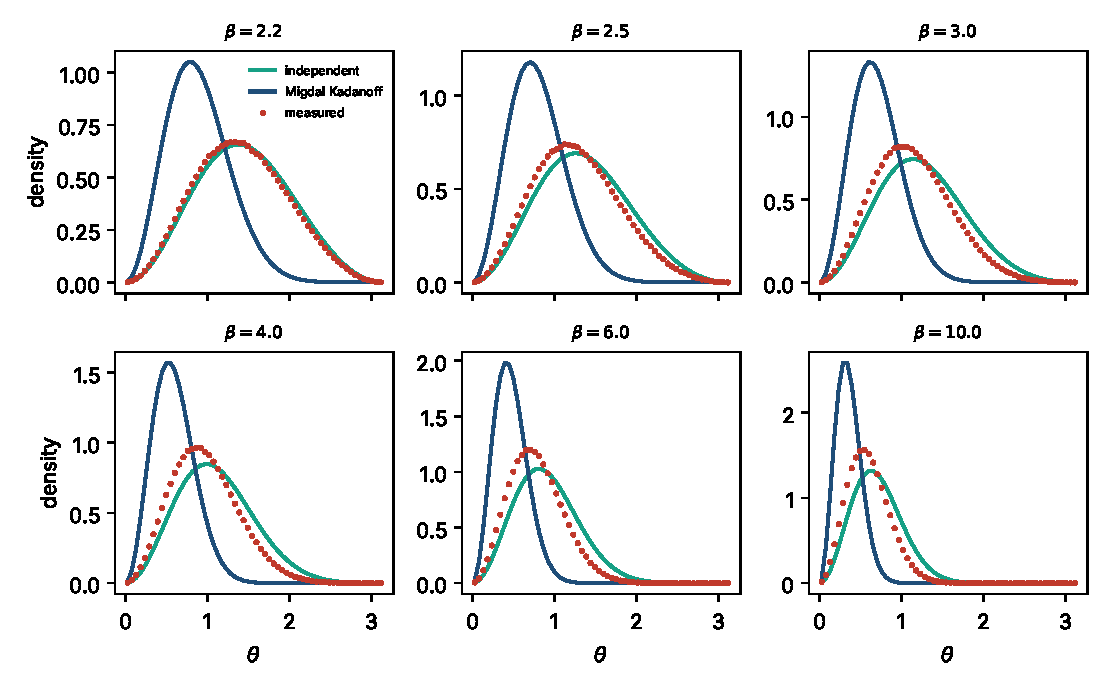
\includegraphics[width=\textwidth]{figures/sandwich.pdf}
\caption[An empirical sandwich for the blocked plaquette]{The law of the rotation angle of the $2\times2$ loop holonomy in four dimensional SU(2), measured on an $8^4$ lattice, between the law for independent plaquettes and the Migdal Kadanoff law, both built from the measured single plaquette law, at six couplings.}
\label{fig:sandwich}
\end{figure}

At every coupling the measured value lies strictly between the other two (Figure~\ref{fig:sandwich}). The last column is the ratio of the logarithms of the $2\times2$ loop and the plaquette. Independent plaquettes would give $4$; the Gaussian ledger of the ladder gives $1$; the simulation gives $3.5$ at the crossover, falling to $2.8$ at weak coupling (here $\beta$ up to $10$).

\section{The likelihood ratio order}

Beyond the means, the sandwich holds in the likelihood ratio order on most of the mass. We computed the two density ratios, independent over measured and measured over Migdal Kadanoff, on the sixty bins of the histograms. If each is increasing in $\theta$, then
\[
\text{Migdal Kadanoff}\ \le_{\mathrm{lr}}\ \text{measured}\ \le_{\mathrm{lr}}\ \text{independent}
\]
in the likelihood ratio order on the angle, to the extent that the ratios are increasing. Weighting bins by the measured mass, the ratio of measured to Migdal Kadanoff is increasing on all of the mass at every coupling. The ratio of independent to measured is increasing on all of the mass for $\beta\ge4$, on $97$ percent at $\beta=2.5$ and $3$, and on $84$ percent at $\beta=2.2$, where the two laws are close and the histogram noise is comparable to their difference. The order is therefore a measured property of most of the mass, not of every bin, and we do not claim it for whole laws.

This is the order in which Chapter~\ref{ch:path} proposed to state the comparison, because bond moving preserves it, and convolution preserves it under the condition of Theorem~\ref{thm:tp2}, which bond moved heat kernel laws satisfy on the near hemisphere $(0,\pi/2]$ (Theorem~\ref{thm:hemisphere}) and, to leading order and numerically, away from a cap at the antipode.

\section{How independent are plaquettes?}

The Migdal Kadanoff approximation and the independent caricature both treat plaquettes at one scale as independent. We measured the correlation of $\frac12\operatorname{tr}U_p$ between neighbouring plaquettes in the same runs.

\begin{center}
\small
\begin{tabular}{cp{1.1in}p{1.1in}p{1.1in}}
\toprule
$\beta$ & same plane, sharing a link & parallel, one step apart & orthogonal planes, sharing a link \\ \midrule
2.2 & 0.010 & 0.035 & 0.043 \\
2.5 & 0.013 & 0.027 & 0.045 \\
4 & 0.017 & 0.021 & 0.046 \\
10 & 0.018 & 0.021 & 0.046 \\
\bottomrule
\end{tabular}
\end{center}

Every correlation is below five percent, at every coupling. Plaquettes are pairwise almost independent, in a loose sense of propagation of chaos, and yet the $2\times2$ loop is far from the product of four independent plaquettes: its logarithm is $2.8$ to $3.5$ times that of a plaquette and not $4$ times. Weak pairwise correlations of one sign, summed coherently over the many plaquettes that touch the loop, produce an effect of order one. That is the content of bond moving, and it explains why the independent caricature fails although pairwise independence nearly holds.

\section{Two steps, and three dimensions}

The same test can be iterated and moved to three dimensions. We measured the laws of the plaquette, the $2\times2$ loop and the $4\times4$ loop, on an $8^4$ lattice at four couplings and on a $16^3$ lattice at four couplings, with a hundred sweeps of equilibration and eighty measurements. In four dimensions the $4\times4$ loop spans half of the periodic box, which limits what these data can show (see below). In three dimensions bond moving has power $b^{d-2}=2$. For each ensemble there are three comparisons: one step from the plaquette to the $2\times2$ loop; one step from the measured $2\times2$ law to the $4\times4$ loop; and two steps from the plaquette to the $4\times4$ loop, with each caricature applied twice. To place the truth inside the bracket we use
\[
\xi=\frac{\log u_2^{\mathrm{meas}}-\log u_2^{\mathrm{ind}}}{\log u_2^{\mathrm{MK}}-\log u_2^{\mathrm{ind}}},
\]
which is $0$ for independent plaquettes and $1$ for Migdal Kadanoff.

\begin{center}
\footnotesize
\begin{tabular}{cccccccc}
\toprule
 & & \multicolumn{3}{c}{$u_2$ of the $4\times4$ loop, two steps} & \multicolumn{3}{c}{position $\xi$} \\
$d$ & $\beta$ & indep. & measured & MK & 1 to 2 & 2 to 4 & 1 to 4 \\ \midrule
4 & 2.5 & 0.0011 & 0.026 & 0.648 & 0.28 & 0.48 & 0.49 \\
4 & 3 & 0.0057 & 0.086 & 0.721 & 0.33 & 0.52 & 0.56 \\
4 & 4 & 0.028 & 0.202 & 0.799 & 0.37 & 0.53 & 0.59 \\
4 & 6 & 0.108 & 0.388 & 0.874 & 0.39 & 0.54 & 0.61 \\
3 & 4 & 0.0062 & 0.021 & 0.267 & 0.22 & 0.33 & 0.32 \\
3 & 6 & 0.046 & 0.126 & 0.456 & 0.31 & 0.44 & 0.44 \\
3 & 9 & 0.143 & 0.305 & 0.613 & 0.36 & 0.53 & 0.52 \\
3 & 14 & 0.298 & 0.494 & 0.740 & 0.39 & 0.56 & 0.56 \\
\bottomrule
\end{tabular}
\end{center}

\begin{figure}[t]
\centering
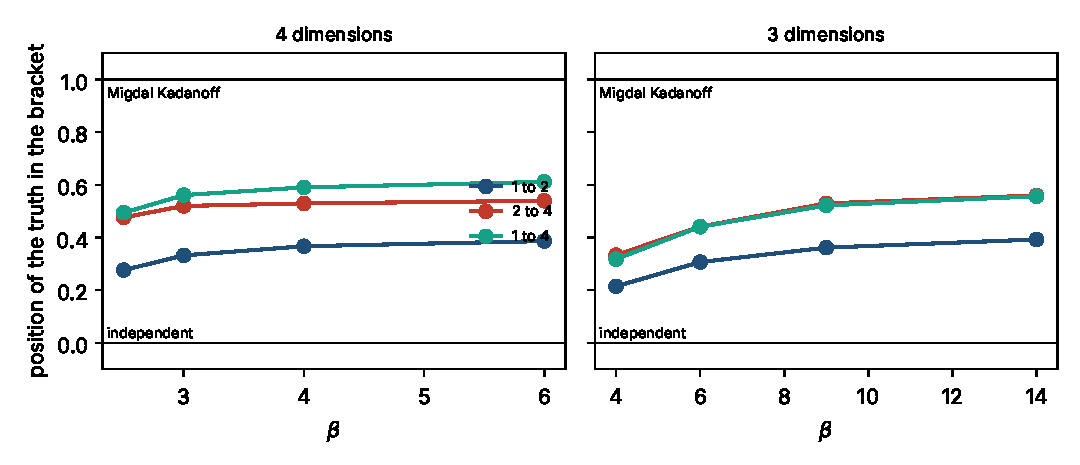
\includegraphics[width=\textwidth]{figures/sandwich2.pdf}
\caption[Position of the truth inside the bracket]{The position $\xi$ of the measured loop law between the independent caricature, $\xi=0$, and the Migdal Kadanoff caricature, $\xi=1$, for one step from the plaquette, one step from the $2\times2$ loop, and two steps, in four and three dimensions.}
\label{fig:sandwich2}
\end{figure}

In all twenty four comparisons the truth lies inside the bracket (Figure~\ref{fig:sandwich2}). The bracket survives a second step: after two applications the caricatures are far apart, a factor of six hundred at $\beta=2.5$ in four dimensions, and the truth sits near the middle on a logarithmic scale. The position drifts upward with the scale, from about $0.35$ at the first step to about $0.55$ at the second, and upward with $\beta$. We read this as a trend in these data only. In four dimensions the $4\times4$ loops live on a periodic $8^4$ lattice, where the loop spans half the box and the runs at $\beta\ge3$ lie above the deconfinement coupling $\beta_c=2.51$ of temporal extent $8$ (Section~\ref{ch:missing}), so finite size effects on these loops are not controlled. Whether the truth moves toward Migdal Kadanoff at larger scales and weaker coupling, as it must if the ladder is to be right about the marginal flow, needs larger lattices. The likelihood ratio order holds on at least $95$ percent of the mass in eighteen of the twenty four comparisons; the exceptions are at the strongest couplings in each dimension, mostly $4\times4$ loops whose laws are within noise of Haar measure.

In three dimensions the bracket is narrower, as Section~\ref{ch:threed} anticipated: at the first step the two caricatures differ by a factor of $1.2$ to $1.9$ in $u_2$, against $1.5$ to $3.7$ in four dimensions.

\section{The sandwich at weak coupling, to leading order}

At weak coupling the three laws can be compared analytically. To lowest order in lattice perturbation theory, in $d$ dimensions,
\[
-\log W_{RR}=\frac{g^2C_F}{2}\int\frac{\mathrm d^dk}{(2\pi)^d}\,F_R(k_\mu)F_R(k_\nu)\,\frac{\hat k_\mu^2+\hat k_\nu^2}{\hat k^2},
\]
where $C_F$ is the quadratic Casimir of the representation, $F_R(k)=\sin^2(kR/2)/\sin^2(k/2)$ and
$\hat k_\rho=2\sin(k_\rho/2)$: the form factor of the $R\times R$ surface against the propagator of the field strength. For $R=1$ the integral is $2/d$, which gives the plaquette $1-3/(4\beta)$ of SU(2) in four dimensions. The ratio $\kappa_R=\log W_{RR}/\log W_{11}$ is then a pure number, the same for every gauge group. We evaluated the momentum sums numerically, in floating point, on lattices up to $32^4$ and $128^3$, with no error bound; the entries below are numerical results for a leading order formula, not theorems.

\begin{center}
\small
\begin{tabular}{cccccc}
\toprule
$d$ & loop & indep. & perturbation theory & MK & position $\xi$ \\ \midrule
4 & $2\times2$ & 4 & 2.739 & 1 & 0.42 \\
4 & $4\times4$ & 16 & 6.523 & 1 & 0.63 \\
3 & $2\times2$ & 4 & 3.120 & 2 & 0.44 \\
3 & $4\times4$ & 16 & 8.715 & 4 & 0.61 \\
\bottomrule
\end{tabular}
\end{center}

The four rows of the table suggest the following statement, which we do not prove.

\begin{conjecture}\label{prop:weaksandwich}
To leading order at weak coupling, in three and four dimensions and for every gauge group, the logarithm of the $2\times2$ and $4\times4$ Wilson loops lies strictly between the values given by independent plaquettes and by the Gaussian ledger of the Migdal Kadanoff ladder.
\end{conjecture}

A proof would need explicit bounds on the infinite volume integrals above.

The simulations approach these limits as they should. In four dimensions the measured ratio $\log W_{22}/\log W_{11}$ is $2.82$ at $\beta=6$ and $2.78$ at $\beta=10$, against $2.735$ for the same sum on an $8^4$ lattice; in three dimensions it is $3.21$ at $\beta=14$ against $3.12$. The measured positions, $0.39$ and $0.61$ in four dimensions at $\beta=6$, are approaching $0.42$ and $0.63$. This also validates the heat bath code against an independent calculation.

At strong coupling the comparison is with the other end of the bracket. A leading order cluster expansion argument, not a proof, gives $W_{22}=W_{11}^4$ to the first orders in $u_2$, because the leading corrections to each side are the same sixteen elementary cubes attached to the same four plaquettes, so the truth approaches the independent caricature, $\xi\to0$, as the data show. The truth therefore travels across the bracket as the coupling weakens, from the independent end toward a limiting position near the middle, and never leaves it in our data. The open part of the problem below is the crossover region, where neither expansion applies.

\section{What the sandwich does and does not show}

It shows that at one step the two caricatures bracket the truth in the right order, at weak coupling, at the crossover and in between. It also locates the truth inside the bracket: in the Gaussian ledger, a bond moving power $k$ gives the ratio $4/k$ in the last column of the first table, so the measured ratios correspond to an effective power between $1.13$ at $\beta=2.2$ and $1.44$ at $\beta=10$, against the ladder's $4$. The ladder overcounts the off plane plaquettes by a factor of about three in this measure, which is the single step form of its misplaced crossover.

It shows the bracket surviving one iteration, at the level of loop laws. It does not show that it survives the iteration that matters, of the effective action. The law of a Wilson loop is not the plaquette law of the blocked effective action: decimation generates couplings of all shapes, and the perimeter self energy of the loop lowers its expectation without lowering the effective coupling. A faithful test iterates a block transformation that keeps the action nearly local, such as the smeared blockings used in Monte Carlo renormalization \cite{Sw79}, fits the plaquette law of each blocked ensemble by the pseudolikelihood of Section~\ref{ch:slice}, and compares rung by rung. The particle ladder of Section~\ref{ch:h6} is the tool for running the two caricatures alongside.

\section{A first empirical rung}

The faithful test described above can be started with the tools already built. We blocked $8^4$ configurations to $4^4$ by two rules, plain decimation, and decimation with the $2\times1$ staples added with weight one half and the sum projected back to SU(2), and fitted a single plaquette Wilson coupling to each ensemble by the pseudolikelihood of Section~\ref{ch:slice}, now with the six staples of four dimensions.

\begin{center}
\small
\begin{tabular}{ccccc}
\toprule
$\beta$ & unblocked & blocked, plain & blocked, smeared & ladder $R(\beta)$ \\ \midrule
2.2 & 2.201 & 0.52 & 1.85 & 1.94 \\
2.5 & 2.499 & 0.87 & 2.81 & 2.24 \\
3 & 3.006 & 1.14 & 4.03 & 2.74 \\
4 & 3.992 & 1.55 & 6.37 & 3.74 \\
6 & 6.010 & 2.26 & 11.2 & 5.75 \\
10 & 9.996 & 3.63 & 20.6 & 9.75 \\
\bottomrule
\end{tabular}
\end{center}

The second column is a validation: on the unblocked ensembles pseudolikelihood recovers the simulated coupling to two parts in a thousand. The next two columns are a caution. The coupling fitted to the blocked field depends strongly on the blocking rule: plain decimation gives about $0.36\beta$ from $\beta=2.5$ upward ($0.24\beta$ at $2.2$), far below the fine coupling, and smearing with weight one half gives up to about $2\beta$, above it from $\beta=2.5$ upward. The ladder's prediction lies between them at every coupling from $\beta=2.5$ upward, and so does the value $\beta-0.26$ that asymptotic freedom requires of a blocking that preserves the long distance physics.

Two lessons follow. A single fitted coupling is not a scheme independent description of the blocked theory; a faithful empirical ladder must fit a richer family of plaquette laws, with the character coefficients of Section~\ref{ch:latent} as parameters, or match observables between a blocked large lattice and an unblocked small one, as in Swendsen's Monte Carlo renormalization group \cite{Sw79}. And the blocking rule is itself a dial that moves the blocked law across the bracket, from the independent end at plain decimation toward and past the Migdal Kadanoff end as the smearing grows. Somewhere on that dial there may be a rule whose fitted coupling follows the renormalized trajectory, and the comparison problem can be posed for that rule. Section~\ref{ch:plgbc} selects a candidate rule at a few couplings on $8^4$ lattices, by matching with a trained generator in place of a fitted coupling; it does not show that the rule follows the trajectory.

\section{The independent end is a theorem}

At the level of means the independent end of the sandwich says $W_{22}\ge W_{11}^4$. For $\Z_2$ gauge theory this is Griffiths' second inequality \cite{Gri67}, in the many spin form of Ginibre \cite{Gi70}. For every compact group it follows from reflection positivity: Corollary~\ref{cor:griffiths} of Section~\ref{ch:griffiths} proves $W_{22}\ge W_{12}^2\ge W_{11}^4$ for every character, at every coupling and in every dimension. So the left ends of the brackets in the tables of this chapter are rigorous lower bounds, and the independent caricature is a true lower caricature for expectations. Theorem~\ref{thm:heatbath} of Section~\ref{ch:griffiths} gives a rigorous upper bound of the same form, with bond moving power $2(d-1)$, but acting on the Wilson weight and not on the measured plaquette law. The two rigorous ends therefore act on different laws: the lower on the measured plaquette law, the upper on the Wilson weight. The ladder's power $2^{d-2}$ lies between the two powers, but this is a comparison of powers and not a bracket of one quantity. Indeed the Migdal Kadanoff value of this chapter, which acts on the measured law, exceeds the proved bound $u(2(d-1)\beta)^4$ in four dimensions at the couplings $\beta=2.5,3,4,6,10$ ($0.665,0.733,0.804,0.875,0.927$ against $0.661,0.710,0.775,0.845,0.904$).

\begin{problem}\label{op:ineq1}
Prove that in SU(2) lattice gauge theory with the Wilson action the law of the $2\times2$ loop holonomy dominates, in the likelihood ratio order, the Migdal Kadanoff law built from the plaquette law, and that both halves of the sandwich hold in the likelihood ratio order. The Migdal Kadanoff end would be a first rigorous comparison between the lattice theory and the ladder at intermediate coupling, for the measured law. At the level of means and at those five couplings, the numbers above already put the measured $2\times2$ mean below the Migdal Kadanoff mean, and the proved bound of Theorem~\ref{thm:heatbath} lies below it too, so the new content of a proof would be the likelihood ratio order and the bound at every coupling.
\end{problem}

\section{Correlation Inequalities}\label{ch:griffiths}\index{Griffiths inequality}\index{Ginibre, J.}\index{correlation inequalities}\index{chessboard estimate}

The independent end of the sandwich above is a correlation inequality. This section recalls the inequalities that are known, with proofs short enough to show where commutativity is used, tests the smallest nonabelian case numerically, and states what a proof for SU(2) would need.

\subsection{Griffiths and Ginibre}

For the Ising model with ferromagnetic couplings, Griffiths \cite{Gri67} proved in 1967 that products of spins have nonnegative expectations and are positively correlated:
\[
\langle\sigma_A\rangle\ge0,\qquad\langle\sigma_A\sigma_B\rangle\ge\langle\sigma_A\rangle\langle\sigma_B\rangle,
\]
where $\sigma_A=\prod_{i\in A}\sigma_i$. Ginibre \cite{Gi70} gave in 1970 a general framework that covers plane rotators and other abelian models.

\begin{theorem}[Ginibre]\label{thm:ginibre}
Let $G$ be a compact abelian group with Haar measure, and $Q$ a convex cone of real continuous functions on $G^n$ that is closed under products and such that for all $f_1,\dots,f_m\in Q$ and all signs,
\[
\int\!\!\int\prod_{i=1}^m\big(f_i(x)\pm f_i(y)\big)\,\mathrm dx\,\mathrm dy\ge0 .
\]
If $-H\in Q$, then under the Gibbs measure $e^{-H}\mathrm dx/Z$, every $f,g\in Q$ satisfy $\langle f\rangle\ge0$ and $\langle fg\rangle\ge\langle f\rangle\langle g\rangle$.
\end{theorem}

\begin{proof}
Duplicate the system, with independent copies $x$ and $y$. Then
\[
2Z^2\big(\langle fg\rangle-\langle f\rangle\langle g\rangle\big)=\int\!\!\int\big(f(x)-f(y)\big)\big(g(x)-g(y)\big)\,e^{-H(x)-H(y)}\,\mathrm dx\,\mathrm dy .
\]
Expand the exponential in powers of $-H(x)-H(y)$, which is of the form $h(x)+h(y)$ with $h\in Q$; since $Q$ is a cone closed under products, each power is a combination with nonnegative coefficients of products of factors $h_j(x)+h_j(y)$. Every term of the expansion is an integral of a product of factors $f_i(x)\pm f_i(y)$ with $f_i\in Q$, hence nonnegative. The same expansion applied to $2Z^2\langle f\rangle=\int\!\!\int\big(f(x)+f(y)\big)e^{-H(x)-H(y)}\,\mathrm dx\,\mathrm dy$ gives $\langle f\rangle\ge0$.
\end{proof}

For the group $\Z_2$ the cone is generated by the products $\sigma_A$; for U(1) by the functions $\cos(\sum_im_i\theta_i)$. The hypothesis of the theorem is checked in the rotated variables: for U(1),
\begin{align*}
\cos a+\cos b&=2\cos\frac{a+b}{2}\cos\frac{a-b}{2},\\
\cos a-\cos b&=2\sin\frac{a+b}{2}\sin\frac{b-a}{2},
\end{align*}
so in the variables $(\theta_i+\theta_i')/2$ and $(\theta_i-\theta_i')/2$ every factor splits into a function of the half sums times the same function of the half differences, up to a reflection that preserves Haar measure, and the double integral factors into a square. That step is where the group must be abelian: it uses the change of variables to sums and differences of the two copies, which is a homomorphism only for a commutative group.

\subsection{Gauge theories}

A lattice gauge theory with group $\Z_2$ or U(1) and Wilson action is of Ginibre's form: the action is a positive combination of plaquette characters, and Wilson loops are characters of products of link variables. Two consequences are classical and follow from Theorem~\ref{thm:ginibre}. Every Wilson loop is nondecreasing in every plaquette coupling. And, switching off all plaquettes outside the plane of a loop, the loop is bounded below by its value in the two dimensional theory, $W_{RT}\ge u^{RT}$ with $u$ the two dimensional plaquette, which bounds the string tension above.

The inequality of the sandwich is stronger: it compares the loop with a power of the plaquette of the same theory. For $\Z_2$, where the plaquette variable is a sign and the loop is literally the product of the four signs inside it, $W_{22}\ge W_{11}^4$ is Griffiths' second inequality applied three times. For U(1) the cosine of a sum of plaquette angles is not the product of the cosines, and we do not know whether the product form follows from Ginibre's theorem.

For nonabelian groups the duplicate variable argument has no analogue, since $(U,U')\mapsto(UU',UU'^{-1})$ does not preserve Haar measure in a useful way and characters of products do not factor; we know of no Ginibre theorem and no FKG inequality, the gap noted in Section~\ref{ch:latent} (the FKG inequality of Fortuin, Kasteleyn and Ginibre~\cite{FKG71}). The inequality of the sandwich nonetheless follows from reflection positivity, in three lines, for every compact gauge group.

\subsection{The inequality is a theorem}

Let $\Pi$ be a lattice hyperplane through sites, $r$ the reflection in it, and $\Theta F=\overline{F\circ r}$. For the Wilson action with $\beta\ge0$, Osterwalder and Seiler's reflection positivity \cite{OSe} holds for this reflection: $\langle F\,\Theta F\rangle\ge0$ for every function $F$ of the links in the closed half space on one side of $\Pi$, the links in $\Pi$ included. The form $(F,G)\mapsto\langle F\,\Theta G\rangle$ is therefore a positive semidefinite inner product and satisfies the Schwarz inequality.

\begin{theorem}[doubling inequality]\label{thm:doubling}
Let $G$ be a compact group, $\rho$ an irreducible unitary representation of dimension $d_\rho$, and $C$ a closed lattice path in the closed half space on one side of $\Pi$ that starts and ends at a site $x\in\Pi$. Let $C\#rC$ be the closed path that follows $C$ and then the reflection of $C$ backwards. Then, for the Wilson action at any $\beta\ge0$ and in any dimension,
\[
\Big|\frac{\langle\chi_\rho(U_C)\rangle}{d_\rho}\Big|^2\ \le\ \frac{\langle\chi_\rho(U_{C\#rC})\rangle}{d_\rho}.
\]
\end{theorem}

\begin{proof}
Let $F_{ab}=\rho(U_C)_{ab}$, a function of the links on one side. By gauge invariance at $x$, the matrix $\langle\rho(U_C)\rangle$ commutes with $\rho(g)$ for every $g$, so by Schur's lemma $\langle F_{ab}\rangle=\delta_{ab}\,\langle\chi_\rho(U_C)\rangle/d_\rho$. The Schwarz inequality with the constant function gives $|\langle F_{ab}\rangle|^2=|\langle F_{ab}\,\Theta1\rangle|^2\le\langle F_{ab}\,\Theta F_{ab}\rangle$. Summing over $a$ and $b$,
\begin{align*}
\frac{\langle\chi_\rho(U_C)\rangle^2}{d_\rho}&\le\Big\langle\sum_{a,b}\rho(U_C)_{ab}\,\overline{\rho(U_{rC})_{ab}}\Big\rangle\\
&=\big\langle\operatorname{tr}\rho\big(U_C\,U_{rC}^{-1}\big)\big\rangle=\langle\chi_\rho(U_{C\#rC})\rangle .
\end{align*}
\end{proof}

If $C$ runs along $\Pi$ for part of its length, that part cancels in $C\#rC$. Take $C$ a plaquette with one edge in $\Pi$: then $C\#rC$ is the $1\times2$ loop. Take $C$ the $1\times2$ loop with its long edge in $\Pi$: then $C\#rC$ is the $2\times2$ loop.

\begin{corollary}\label{cor:griffiths}
For every compact gauge group, every $\beta\ge0$, every dimension and every irreducible representation, with normalised characters,
\[
W_{12}\ge W_{11}^2,\qquad W_{22}\ge W_{12}^2\ge W_{11}^4,\qquad W_{2^p\times2^q}\ge W_{11}^{2^{p+q}} .
\]
In particular, along loops $2^p\times2^q$, the string tension satisfies $\sigma a^2\le-\log W_{11}$, and for SU(2) every character coefficient of the law of the $2\times2$ loop holonomy is at least that of the law built from four independent plaquettes: $u_n^{\mathrm{meas}}\ge(u_n^{\mathrm{plaq}})^4$ for all $n$.
\end{corollary}

The independent end of the sandwich is thus a theorem at the level of every character, at every coupling, including the crossover. It is a classical kind of statement, in the family of the loop inequalities derived from reflection positivity since the late 1970s, which also give the convexity of the static potential \cite{Ba86}. What the theorem does not give is the likelihood ratio order between the two laws, which is a statement about all characters jointly, and it says nothing about the Migdal Kadanoff end.

The proof also explains the numbers. The inequality is a Schwarz inequality between the plaquette and the constant function in the reflection positive inner product, so the deficit $W_{12}-W_{11}^2$ is the squared norm of the component of the plaquette orthogonal to the vacuum, transported across the plane: a sum over excited states $\sum_{E>0}|c_E|^2$ with the weights of the spectral measure of Chapter~\ref{ch:positivity}. It vanishes in two dimensions, where the link in $\Pi$ carries no excitations between the two plaquettes, and it is small at strong coupling, where correlations across the plane are weak.

\subsection{The smallest nonabelian test}

The simulations below were run before we had the theorem, as a test of a conjecture; they now serve as a check of the code and as a measurement of the deficit. The smallest case is two adjacent plaquettes, $W_{12}\ge W_{11}^2$. In two dimensions equality holds, because the plaquettes are independent. In four dimensions we measured both sides on an $8^4$ lattice, forty configurations five sweeps apart at each coupling.

\begin{center}
\small
\begin{tabular}{ccccc}
\toprule
$\beta$ & $W_{12}$ & $W_{11}^2$ & difference & standard error \\ \midrule
2.2 & 0.3424 & 0.3251 & 0.0173 & 0.0003 \\
2.5 & 0.4586 & 0.4265 & 0.0321 & 0.0002 \\
3 & 0.5602 & 0.5241 & 0.0362 & 0.0002 \\
4 & 0.6735 & 0.6392 & 0.0343 & 0.0002 \\
6 & 0.7841 & 0.7572 & 0.0269 & 0.0001 \\
10 & 0.8707 & 0.8526 & 0.0181 & 0.0001 \\
\bottomrule
\end{tabular}
\end{center}

The inequality holds at every coupling, by more than fifty standard errors. The difference is largest near $\beta=3$, just above the crossover, and vanishes at both ends: at strong coupling by the cluster property, and at weak coupling because both sides tend to one. In lowest order perturbation theory $\log W_{12}/\log W_{11}=1.724$ in four dimensions, less than two for the same reason that $\log W_{22}/\log W_{11}$ is less than four: the form factor of a larger surface suppresses the high momenta that dominate the plaquette. The resulting prediction, $W_{12}-W_{11}^2=e^{-2w}(e^{0.276w}-1)$ with $w=3/(4\beta)$, is positive at every coupling and describes the data from $\beta=4$ upward (Figure~\ref{fig:griffiths}).

\begin{figure}[t]
\centering
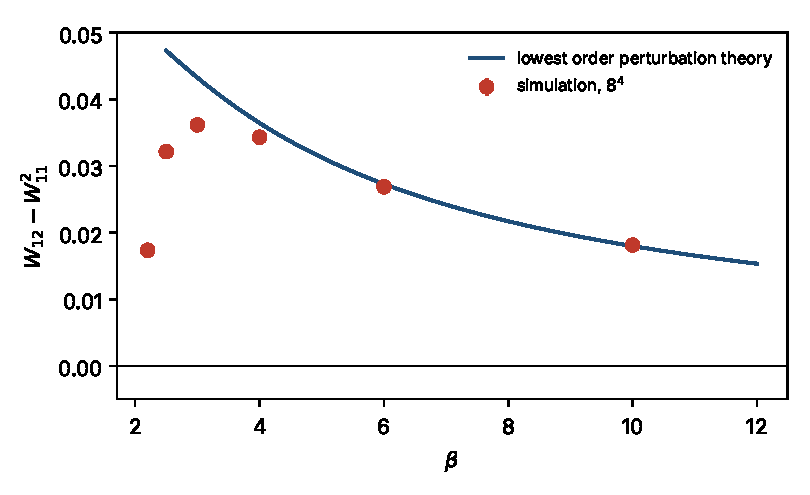
\includegraphics[width=0.8\textwidth]{figures/griffiths.pdf}
\caption[The smallest Griffiths test for SU(2)]{The difference $W_{12}-W_{11}^2$ for four dimensional SU(2) on an $8^4$ lattice, with bars of three standard errors, and the prediction of lowest order perturbation theory. The difference is positive at every coupling.}
\label{fig:griffiths}
\end{figure}

\subsection{The strong coupling side}

The table above stops at the crossover. Below it the difference is small and needs more statistics. We ran four hundred configurations at each of five strong couplings.

\begin{center}
\small
\begin{tabular}{cccc}
\toprule
$\beta$ & $W_{11}$ & $W_{12}-W_{11}^2$ & standard error \\ \midrule
1.2 & 0.290 & 0.00032 & 0.00010 \\
1.4 & 0.338 & 0.00042 & 0.00011 \\
1.6 & 0.388 & 0.00113 & 0.00009 \\
1.8 & 0.441 & 0.00327 & 0.00014 \\
2.0 & 0.501 & 0.00757 & 0.00009 \\
\bottomrule
\end{tabular}
\end{center}

The difference is positive at every coupling, by three standard errors at $\beta=1.2$ and by more than twelve from $\beta=1.6$ upward. It falls steeply, roughly like the eighth power of the plaquette, which is the order at which the strong coupling expansions of the two sides first differ: to order $u^6$ both are $u^2$ plus the same elementary cubes attached to the same two plaquettes, and at order $u^8$ the loop has surfaces spanning both plaquettes at once that the product does not. A naive count of those surfaces gives $2(d-2)u^8$; the data are about half of that between $\beta=1.4$ and $2$, so terms with higher representations contribute at the same order with the opposite sign, and we have not computed the coefficient. With the six couplings from the crossover upward, the inequality has been checked at eleven couplings from $\beta=1.2$ to $\beta=10$.

\subsection{A rigorous upper bound}

The other side has a classical answer too, of a different kind. Integrate out some of the links of the loop exactly.

\begin{theorem}[heat bath bound]\label{thm:heatbath}
Let $C$ be a closed lattice path without repeated links, and $A$ a set of links of $C$ no two of which lie in a common plaquette. For SU(2) with the Wilson action in $d$ dimensions, with $u(x)=I_2(x)/I_1(x)$ and $V_\ell$ the sum of the $2(d-1)$ staples of the link $\ell$,
\[
|W_C|\ \le\ \Big\langle\prod_{\ell\in A}u\big(\beta|V_\ell|\big)\Big\rangle\ \le\ u\big(2(d-1)\beta\big)^{|A|}.
\]
For an $R\times T$ rectangle with $R,T\ge2$ one can take $|A|=2R+2T-4$. In particular
\[
W_{11}^4\ \le\ W_{22}\ \le\ u\big(2(d-1)\beta\big)^4 .
\]
\end{theorem}

\begin{proof}
Every plaquette contains at most one link of $A$, so given all other links the links of $A$ are independent, each with density proportional to $\exp(\beta\,\frac12\operatorname{tr}(U_\ell V_\ell))$, and the staple sums $V_\ell$ do not involve links of $A$. A sum of elements of SU(2) is a nonnegative multiple of an element of SU(2), $V_\ell=|V_\ell|\hat V_\ell$, and the conditional mean of $U_\ell$ is $u(\beta|V_\ell|)\,\hat V_\ell^{-1}$, by the single link computation of Section~\ref{ch:slice}. The trace of the holonomy is linear in each link of $A$. Taking the conditional expectation replaces each such link by its conditional mean, which leaves the normalised trace of an element of SU(2), of modulus at most one, times the product of the factors $u(\beta|V_\ell|)$. Finally $|V_\ell|\le2(d-1)$ and $u$ is increasing. For the rectangle, collinear links and links on opposite sides at distance at least two share no plaquette; dropping one link at each corner removes the corner plaquettes.
\end{proof}

The first inequality is the multihit estimator of Parisi, Petronzio and Rapuano \cite{PPR}, which lattice practitioners use to reduce the variance of Wilson loops; in statistical language it is Rao Blackwellisation~\cite{Bl47}, and the theorem is the remark that a Rao Blackwellised estimator bounded by a product of positive factors gives an inequality. The second is a perimeter bound of a classical kind.

Together with Corollary~\ref{cor:griffiths} it gives a rigorous sandwich for expectations, and both ends are caricatures of Migdal Kadanoff type: products of plaquette weights followed by a convolution of four. They act on different laws, as the table says.
\begin{center}
\small
\begin{tabular}{p{1.4in}p{1.35in}p{1.35in}}
\toprule
caricature & bond moving power & status \\ \midrule
independent plaquettes & $1$, on the measured law & rigorous lower bound \\
truth, by the ratio of logarithms & $1.1$ to $1.4$ & measured \\
Migdal Kadanoff, $b=2$ & $2^{d-2}$, on the Wilson weight & conjectured upper bound \\
heat bath bound & $2(d-1)$, on the Wilson weight & rigorous upper bound \\
\bottomrule
\end{tabular}
\end{center}
In four dimensions the powers are $1$, $4$ and $6$; in three, $1$, $2$ and $4$; in two, $1$, $1$ and $2$. The ladder's power lies between the two rigorous powers in every dimension, and in two dimensions it coincides with the lower end and with the truth. This compares powers on different laws: the lower end acts on the measured plaquette law, the upper on the Wilson weight, and the Migdal Kadanoff step on the measured law of the first half of this chapter lies above the upper bound for $\beta\ge2.5$ in four dimensions.

We measured all five quantities in separate runs on the same lattices; they agree with the tables of the first half of this chapter to two units in the third decimal.

\begin{center}
\footnotesize
\begin{tabular}{ccccccc}
\toprule
$d$ & $\beta$ & $W_{11}^4$ & $W_{22}$ & $u(2^{d-2}\beta)^4$ & $\langle\prod u(\beta|V_\ell|)\rangle$ & $u(2(d-1)\beta)^4$ \\ \midrule
4 & 2.2 & 0.105 & 0.136 & 0.486 & 0.480 & 0.624 \\
4 & 2.5 & 0.181 & 0.259 & 0.532 & 0.567 & 0.661 \\
4 & 3 & 0.274 & 0.379 & 0.594 & 0.649 & 0.710 \\
4 & 4 & 0.409 & 0.525 & 0.679 & 0.742 & 0.775 \\
4 & 6 & 0.572 & 0.675 & 0.775 & 0.830 & 0.845 \\
4 & 10 & 0.727 & 0.801 & 0.859 & 0.899 & 0.904 \\
3 & 4 & 0.280 & 0.323 & 0.451 & 0.618 & 0.679 \\
3 & 6 & 0.463 & 0.522 & 0.594 & 0.748 & 0.775 \\
3 & 9 & 0.615 & 0.673 & 0.710 & 0.833 & 0.845 \\
3 & 14 & 0.740 & 0.785 & 0.804 & 0.893 & 0.898 \\
\bottomrule
\end{tabular}
\end{center}

The rigorous chain $W_{11}^4\le W_{22}\le\langle\prod u\rangle\le u(2(d-1)\beta)^4$ holds in every row, as it must. The middle column is the first step of the ladder from the Wilson weight itself, $u(2^{d-2}\beta)^4$. It lies above the measured loop in all ten rows.

\begin{problem}\label{op:ineq2}
Prove the bare form of the Migdal Kadanoff end of the sandwich: for SU(2) with the Wilson action in $d$ dimensions and every $\beta\ge0$,
\[
W_{22}(\beta)\ \le\ \Big(\frac{I_2(2^{d-2}\beta)}{I_1(2^{d-2}\beta)}\Big)^4 .
\]
\end{problem}

The inequality is an equality in two dimensions. It holds at strong coupling, where the left side is $(\beta/4)^4$ and the right side $(2^{d-2}\beta/4)^4$ to leading order. At weak coupling, lowest order perturbation theory gives $-\log W_{22}=2.054/\beta$ in four dimensions and $3.120/\beta$ in three, against $1.5/\beta$ and $3/\beta$ for the right side: it holds with room in four dimensions and by four percent in three. That near equality says something: in three dimensions the bond moving power $b^{d-2}$ is close to the sharpest constant for which such a bound can hold at weak coupling. The heat bath bound proves the inequality with $2(d-1)$ in place of $2^{d-2}$; the gap between them is the difference between counting all the plaquettes at a link and counting only those that Migdal and Kadanoff move. The measured column $\langle\prod u(\beta|V_\ell|)\rangle$ shows why the heat bath argument alone cannot close it: at $\beta=2.5$ the effective staple sum, with length defined by inverting the measured value, has length about $4.5$ in four dimensions, between $4$ and $6$.

\subsection{Why the bound cannot be iterated naively}

The problem above is about the $2\times2$ loop and one step. Its obvious extension, $W_{RR}(\beta)\le u(2^{d-2}\beta)^{R^2}$, which would say that the theory in $d$ dimensions is bounded by the two dimensional theory at the bond moved coupling for every loop, fails in our data and in lowest order perturbation theory, and it is instructive to see how.

\begin{center}
\small
\begin{tabular}{cccc}
\toprule
$d$ & $\beta$ & $W_{44}$ measured & $u(2^{d-2}\beta)^{16}$ \\ \midrule
4 & 2.5 & 0.026 & 0.080 \\
4 & 4 & 0.202 & 0.213 \\
4 & 6 & 0.388 & 0.360 \\
3 & 4 & 0.021 & 0.041 \\
3 & 6 & 0.126 & 0.124 \\
3 & 14 & 0.494 & 0.418 \\
\bottomrule
\end{tabular}
\end{center}

The bound fails for the $4\times4$ loop at $\beta=6$ in four dimensions and from $\beta=6$ upward in three. It should: at weak coupling the logarithm of a loop grows with its perimeter (compare Theorem~\ref{thm:heatbath}), while the two dimensional expression grows with its area, and in perturbation theory $-\log W_{44}=4.89/\beta$ in four dimensions against $6/\beta$ for the bound. For very large loops the same failure is the statement that the string tension at weak coupling is exponentially small and not of order $1/\beta$. The abelian control of Section~\ref{ch:missing} says the same thing more sharply: in a theory with a deconfined phase no area law bound can hold for large loops.

So a comparison with the ladder cannot be a comparison of Wilson loops of the original theory with a fixed two dimensional theory. One step of scale two can be compared loop by loop; after that the coupling has moved, and the next comparison must be made for the blocked theory at its own coupling. This is the content of renormalization, and it is the reason the sandwich has to be stated for the law of the blocked plaquette of an effective action and not for large loops.

\subsection{Kadanoff's bound: the whole ladder is rigorous for the pressure}

There is one inequality that does iterate, and it is also classical \cite{Ka75,Ka76}. Let
\[
P(\beta)=\lim\frac{1}{\#\text{plaquettes}}\log\int\prod_pe^{\beta\cos\theta_p}\prod_\ell\mathrm dU_\ell
\]
be the pressure per plaquette, so that $P'(\beta)=W_{11}(\beta)$.

\begin{theorem}[Kadanoff]\label{thm:kadanoff}
Let $\nu_m$ be the normalised plaquette law at rung $m$ of the Migdal Kadanoff ladder with scale factor $b$ in $d$ dimensions, started from the Wilson law, and $k=b^{d-2}$. Then
\[
P(\beta)\ \le\ P_{\mathrm{MK}}(\beta)=\log\frac{2I_1(\beta)}{\beta}+\frac1k\sum_{m\ge0}b^{-dm}\log\int\nu_m^k\,\mathrm d\mathrm{Haar}.
\]
\end{theorem}

\begin{proof}
Bond moving replaces the action $S$ by an action $S'$ in which plaquette terms have been transferred between parallel plaquettes with the total coupling unchanged. By lattice symmetry every plaquette term has the same expectation under the original measure, so $\langle S'-S\rangle=0$, and by Jensen's inequality $Z'/Z=\langle e^{-(S'-S)}\rangle\ge e^{-\langle S'-S\rangle}=1$. In the moved system the links freed by the move are integrated exactly, which convolves the moved plaquette weights; each of the $\#\text{plaquettes}/k$ weights $\nu^k$ contributes its normalisation, and what remains is the partition function of a lattice coarser by the factor $b$ with the law of the next rung. That lattice is again symmetric, and the argument repeats.
\end{proof}

This is a rigorous statement that relates the entire ladder, every rung, to the theory on $\Z^d$. Since $P(0)=0$ and $P'=W_{11}$, it bounds the integral of the plaquette over the coupling. We evaluated both sides in four dimensions, the left from our measured plaquettes and the right from the ladder (Figure~\ref{fig:kadanoff}).

\begin{center}
\small
\begin{tabular}{ccccc}
\toprule
$\beta$ & $P$ in two dimensions & $P$, measured & $P_{\mathrm{MK}}$ & heat bath \\ \midrule
1 & 0.123 & 0.123 & 0.407 & \\
2.5 & 0.700 & 0.780 & 1.628 & 1.781 \\
4 & 1.585 & 1.892 & 2.986 & 3.165 \\
10 & 6.281 & 7.185 & 8.710 & \\
\bottomrule
\end{tabular}
\end{center}

\begin{figure}[t]
\centering
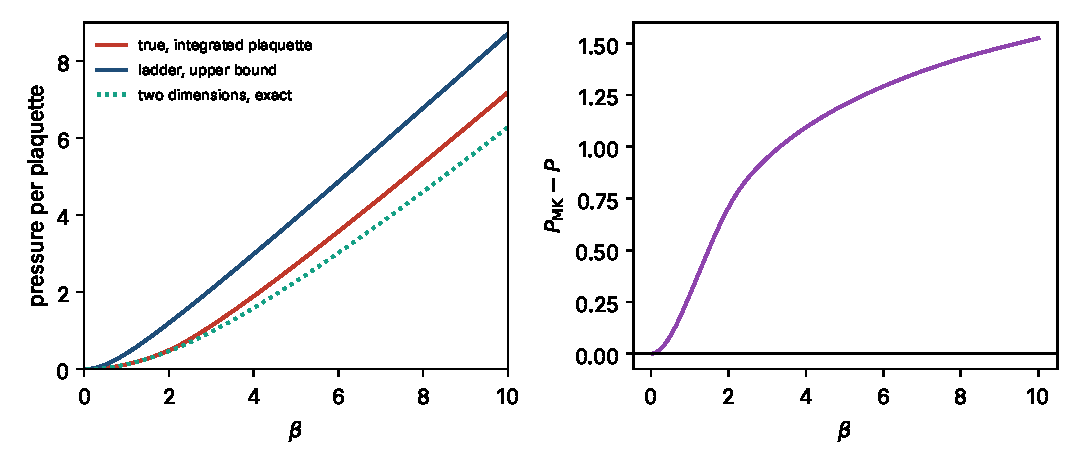
\includegraphics[width=\textwidth]{figures/kadanoff_bound.pdf}
\caption[Kadanoff's bound on the pressure]{Left: the pressure per plaquette of four dimensional SU(2), obtained by integrating the measured plaquette, the rigorous upper bound from the Migdal Kadanoff ladder, and the exact two dimensional pressure. Right: the gap between the ladder's bound and the truth.}
\label{fig:kadanoff}
\end{figure}

The bound holds, with a gap that grows slowly, from $0.3$ at $\beta=1$ to $1.5$ at $\beta=10$: at weak coupling both pressures grow like $\beta$ minus a multiple of $\log\beta$, with different multiples. The ladder's bound is a little better than the one obtained by integrating the heat bath bound $W_{11}\le u(2(d-1)\beta)$. The true pressure lies above the two dimensional one in every row (equal to three decimals at $\beta=1$), the integrated form of an inequality, $W_{11}^{(d)}\ge W_{11}^{(2)}$, that Ginibre's theorem gives for abelian groups and that is open for SU(2).

Kadanoff's bound is too weak to give a gap: a bound on a pressure does not bound a correlation length. But it fixes the direction of the ladder's error rigorously and at every scale. The moved system has more pressure than the true one; it is stiffer. Every numerical comparison in this chapter found the ladder on that side.

\subsection{What remains}

Three things. The bare inequality above, which would make the ladder's first step a rigorous upper caricature. The order between laws: the corollary and the theorem bound expectations, character by character on the independent side, and the likelihood ratio order supported by the data of the first half of this chapter asks for more. And iteration: a sandwich for expectations at one step does not control the next step unless it holds between laws in an order that the two operations of the ladder preserve, which is where Theorem~\ref{thm:tp2} and the bad cap enter.

\section*{Exercises}
\begin{enumerate}
\item Show that in two dimensions the measured and independent laws of the first section of this chapter coincide.
\item Show that in the Gaussian ledger a bond moving power $k$ followed by decimation with $b=2$ gives $\log W_{22}/\log W_{11}=4/k$.
\item Prove $W_{22}\ge W_{11}^4$ for $\Z_2$ gauge theory from Griffiths' second inequality (Section~\ref{ch:griffiths}).
\item Prove Griffiths' first inequality for the Ising model by expanding $e^{J\sigma_i\sigma_j}=\cosh J\,(1+\sigma_i\sigma_j\tanh J)$.
\item Verify the identity for $\cos a\pm\cos b$ and complete the proof of Theorem~\ref{thm:ginibre} for the plane rotator.
\item Show that in two dimensional SU(2) lattice gauge theory $W_{12}=W_{11}^2$, and identify the step of the proof of Theorem~\ref{thm:doubling} that is an equality there.
\item Use the proof of Theorem~\ref{thm:doubling}, with the Schwarz inequality for two different functions, and a plane that cuts a rectangular loop to prove $W_{R_1+R_2,T}^2\le W_{2R_1,T}\,W_{2R_2,T}$, the convexity of the static potential.
\item Extend Theorem~\ref{thm:heatbath} to SU(N), replacing $u$ by the mean of the fundamental character under the single link conditional (for SU(N) that conditional mean is not a scalar times a group element, so operator norms may be needed).
\item Compute $\log W_{12}/\log W_{11}$ in lowest order perturbation theory in four dimensions with the code of Appendix~\ref{ch:code}, extended from square to rectangular loops.
\end{enumerate}
